\documentclass{article}
\usepackage[utf8]{inputenc}
\usepackage[a4paper,top=2cm,bottom=2cm,left=3cm,right=3cm,marginparwidth=1.75cm]{geometry}
\usepackage{amsmath}
\usepackage{graphicx}
\usepackage{subfig}
\usepackage[colorlinks=true, allcolors=blue]{hyperref}

\begin{document}

\begin{titlepage}

\center % Center everything on the page

\newcommand{\HRule}{\rule{\linewidth}{0.4mm}} % Barra horizontal

\begin{figure}[h!]
    \centering
    
\includegraphics[width=0.24\linewidth]{images/uniMinho.jpg}
\end{figure}

%\textsc{\Large Universidade do Minho}\\[0.75cm]  % Name of your university/college
\textsc{\Large Licenciatura em Ciências da Computação}\\[0.4cm] % Nome do curso
\textsc{\Large Sistemas de Comunicações e Redes}\\[5cm]

{\Large\bfseries Ensaio Escrito}\\[0.5cm]
{\LARGE \bfseries Aplicações e Camada de Transporte} % Título


\vspace{5cm} % Autores
{\bfseries Grupo 28} \\ \vspace{3mm}
Davide Santos (A102938) \\ \vspace{3mm}
Edgar Araújo (A102946) \\ \vspace{3mm}
Pedro Augusto Camargo (A102504) \\ \vspace{3mm}
\vspace{0.2cm}
{Novembro 2023}\\[0.2cm] % Data

\vfill % Fill the rest of the page with whitespace
\end{titlepage}

\tableofcontents
\pagebreak

\section{Nível aplicacional}
\subsection{Identifique o endereço IP da estação que formulou a query DNS e o tipo de query realizada.}
\begin{figure}[h!]
    \centering
    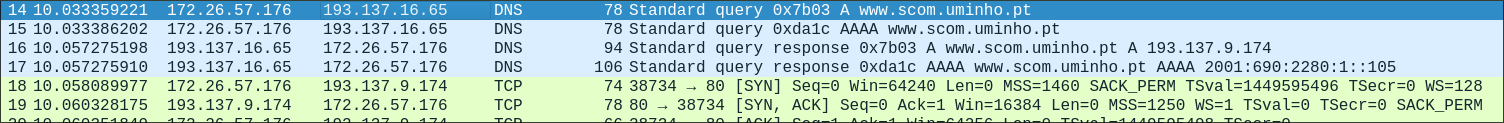
\includegraphics[width=1\linewidth]{images/dns.png}
\end{figure}

O endereço IP da estação que formulou a query DNS: 172.26.57.176 (O meu computador)
Foram enviadas 2 querys dns, uma do tipo A (endereço IPv4) e outra do tipo AAAA (endereço IPv6)

\subsection{Localize a trama com a resposta à query DNS formulada. Identifique nesta trama o endereço IP do
servidor web. Identifique também o servidor de nomes que forneceu a resposta, através do seu IP e nome}

\begin{figure}[h!]
    \centering
    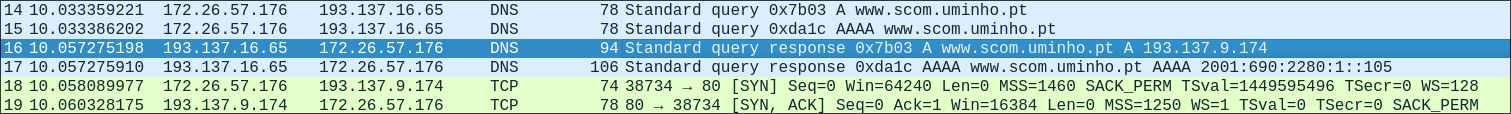
\includegraphics[width=1\linewidth]{images/dns_response.png}
\end{figure}

O endereço IP do servidor web que respondeu a query DNS: 193.137.16.65
De forma a identificar o servidor de nomes que forneceu a resposta, poderia ter sido usado o utilitario nslookup, como tambem o servico WEB https://whatismyipaddress.com/ip/\textless ip\textgreater,
para o ip anterior:
\begin{figure}[h!]
    \centering
    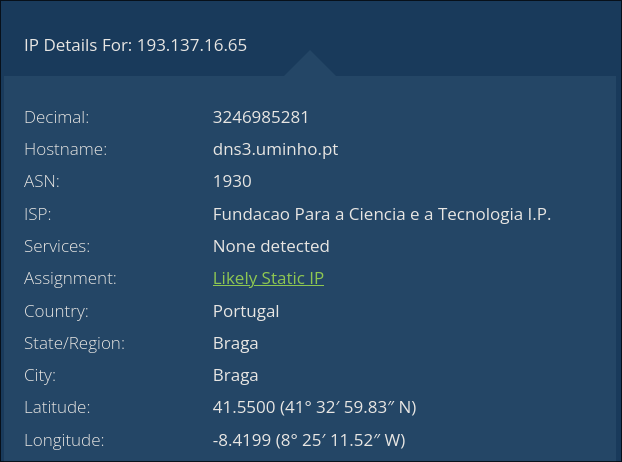
\includegraphics[width=0.5\linewidth]{images/whats.png}
\end{figure}

Obtemos que o servidor DNS que forneceu a resposta, tem por hostname: dns3.uminho.pt

\subsection{Aplique o filtro aos protocolos http // tcp. Identifique os endereços IP do cliente e do servidor HTTP}
\begin{figure}[h!]
    \centering
    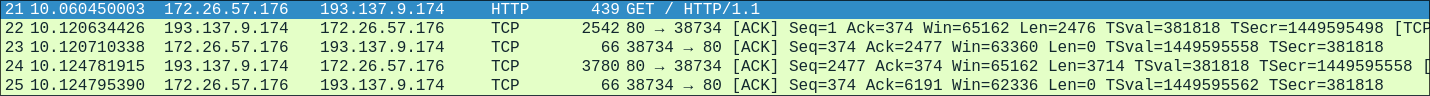
\includegraphics[width=1\linewidth]{images/http_ip.png}
\end{figure}

\begin{itemize}
    \item Temos o endereco IP do cliente, vindo do HTTP GET Request: 172.26.57.176
    \item Que tem como destino o IP do servidor: 193.137.9.174
\end{itemize}

\subsection{Identifique os segmentos TCP correspondentes ao estabelecimento da ligação entre o cliente e o servidor
HTTP. Qual o o tamanho máximo de segmento (MSS) que o servidor aceita receber?}

\begin{figure}[h!]
    \centering
    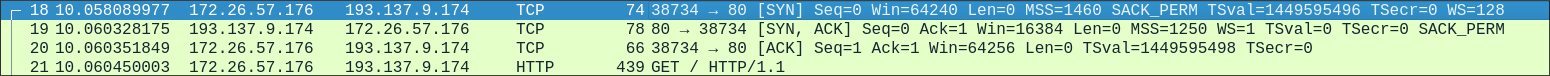
\includegraphics[width=1\linewidth]{images/mss.png}
\end{figure}

Tal como mostra a imagem, os pacotes 18 e 19 correspondem aos pactoes SYN do cliente e SYN-ACK do servidor, respetivamente.
Logo ambos tem oportunidade nestes pacotes de solicitar um MSS, que no caso do servidor é de 1250 bytes.

\subsection{Identifique a resposta HTTP do servidor respeitante ao primeiro pedido GET efetuado pelo cliente.
Quantos bytes de dados aplicacionais contém essa resposta HTTP?}

\begin{figure}[h!]
    \centering
    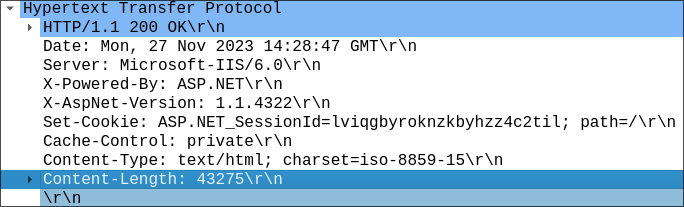
\includegraphics[width=0.5\linewidth]{images/ok.png}
\end{figure}

A resposta HTTP do servidor é do tipo 200 OK, e contem 43275 bytes de dados aplicacionais, tal como indica o campo Content-Length.

\subsection{A resposta HTTP identificada na alínea anterior foi transmitida em quantos segmentos TCP? Apresente
também uma estimativa teórica para essa quantidade.}

\begin{figure}[h!]
    \centering
    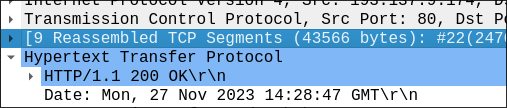
\includegraphics[width=0.5\linewidth]{images/segments.png}
\end{figure}

A resposta HTTP foi transmitida em 9 segmentos. A estimativa teórica para essa quantidade é de 43566/1460 = 29.8, ou seja, 30 segmentos.

\subsection{A partir da informação contida nos cabeçalhos dos protocolos IP e TCP, determine o número de bytes de
dados enviados no primeiro e no último segmento TCP respeitantes à resposta HTTP.}

\begin{figure}[h!]
    \centering
    \subfloat[\centering Primeiro Segmento]{{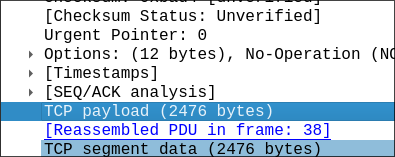
\includegraphics[width=5cm]{images/start.png} }}
    \qquad
    \subfloat[\centering Último Segmento]{{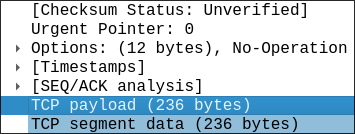
\includegraphics[width=5cm]{images/end.png} }}
\end{figure}

No primeiro segmento TCP, o número de bytes de dados enviados é de 2476 bytes. No último segmento TCP, o número de bytes de dados enviados é de 236 bytes.

\subsection{Observe a informação apresentada no campo host do cabeçalho do pedido HTTP e diga qual o seu
interesse?}

\begin{figure}[h!]
    \centering
    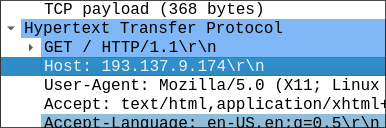
\includegraphics[width=0.5\linewidth]{images/host.png}
\end{figure}

O campo host do cabeçalho do pedido HTTP indica o nome colocado no url do browser, que serve para identificar o website que se pretende aceder, em caso de um servidor conter vários websites diferentes.

\subsection{Com base na sequência de dados trocados entre o cliente e o servidor diga, justificando, se o servidor
HTTP está a funcionar em modo de conexão persistente ou não persistente.}

\begin{figure}[h!]
    \centering
    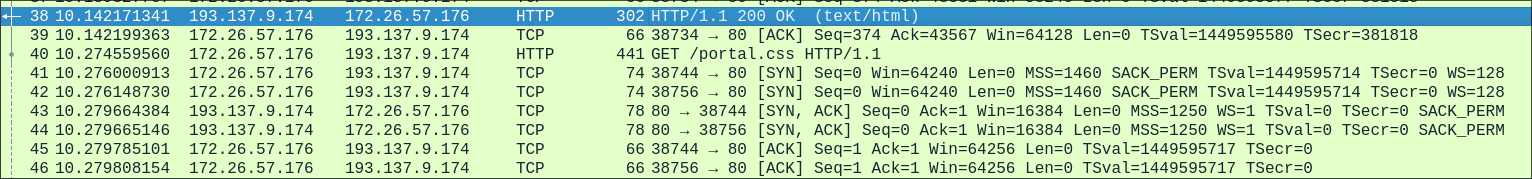
\includegraphics[width=1\linewidth]{images/conexao.png}
\end{figure}

O servidor HTTP está a funcionar em modo de conexão persistente, pois nenhum dos segmentos TCP tem a flag FIN ativa, entre GET Requests.

\subsection{Aceda a https://www.uminho.pt, ao mesmo tempo que captura o tráfego desse acesso com o Wireshark.
Porque razão o tráfego HTTP não é identificado como tal no Wireshark? Apesar disso, pode detetar-se
qual o protocolo aplicacional. Como é que o Wireshark sabe que se trata duma ligação http-over-tls?}

A razao pela qual o trafego HTTP nao é identificado como tal no Wireshark, é porque o trafego HTTP está a ser feito sobre o protocolo TLS, que é um protocolo de segurança que encripta o trafego HTTP, de forma a que este não seja visivel a terceiros. O Wireshark sabe que se trata de uma ligação http-over-tls, porque o protocolo TLS é identificado no campo Protocol do pacote.

\subsection{Diga, justificando, quais dos seguintes elementos uma comunicação HTTPS permite manter ocultos dum
atacante: i) o endereço IP do cliente, ii) o endereço IP do servidor web, iii) o nome do servidor web, iv) o
tamanho da mensagem trocada entre o cliente o servidor, v) a identificação da página acedida no servidor
web, vi) a frequência das conexões estabelecidas entre o cliente e o servidor, vii) os dados da aplicação
trocados entre o servidor e o cliente}

\begin{itemize}
    \item i) O endereço IP do cliente não é oculto, pois é necessário para que o servidor saiba para onde enviar a resposta.
    \item ii) O endereço IP do servidor web não é oculto, pois é necessário para que o cliente saiba para onde enviar o pedido.
    \item iii) O nome do servidor web não é oculto, pois é necessário para que o servidor saiba para que website enviar o pedido.
    \item iv) O tamanho da mensagem trocada entre o cliente e o servidor não é oculto, pois é necessário para que o cliente saiba se recebeu a mensagem completa.
    \item v) A identificação da página acedida no servidor web não é oculto. O caminho do URL é parte da solicitação HTTP e, embora a comunicação seja criptografada, a estrutura básica da solicitação permanece visível.
    \item vi) A frequência das conexões estabelecidas entre o cliente e o servidor não é oculto, pois é necessário para que o servidor saiba se o cliente está a tentar fazer um ataque de negação de serviço.
    \item vii) Os dados da aplicação trocados entre o servidor e o cliente SÃO ocultos, isso garante que o conteúdo da mensagem, incluindo informações sensíveis, não seja visível para um atacante que possa interceptar a comunicação. 
\end{itemize}

\section{Parte 2}
\subsection{Usando o registo MX}
\subsubsection{Quais são os servidores de email do domínio “tecnico.ulisboa.pt.”?}

Utilizando o comando dig MX tecnico.ulisboa.pt, obtemos os seguintes servidores de email:
\begin{itemize}
    \item 51 smtp1.tecnico.ulisboa.pt.
    \item 10 smtp.tecnico.ulisboa.pt.
    \item 61 smtp2.tecnico.ulisboa.pt.
\end{itemize}

\subsubsection{A que sistema são preferencialmente entregues as mensagens dirigidas a
geral@tecnico.ulisboa.pt?}

As mensagens sao preferencialmente entregues ao sistema de maior prioridade, isto e, os de menor numero a esquerda do nome do servidor de email, logo as mensagens seriam entregues ao servidor smtp.tecnico.ulisboa.pt, no caso deste estar indisponivel, a mensagem seria entao entregue ao seguintes, por ordem, smtp1.tecnico.ulisboa.pt e por fim smtp2.tecnico.ulisboa.pt.

\subsection{A resposta obtida a uma query pode ser classificada como autoritativa ou não-autoritativa.}
\subsubsection{Qual a diferença fundamental entre ambos os tipos de resposta?}

A diferença fundamental entre ambos os tipos de resposta é que uma resposta autoritativa é uma resposta que vem diretamente do servidor DNS que contém a informação sobre o domínio, enquanto que uma resposta não-autoritativa é uma resposta que vem de um servidor DNS que não contém a informação sobre o domínio, mas que obteve essa informação de um servidor DNS autoritativo.
Logo enquanto a resposta nao autoritativa pode conter informação desatualizada, a resposta autoritativa contém sempre a informação mais atualizada.

\subsubsection{Usando o seu default DNS server, que tipos de resposta obtém se efetuar queries aos registos
MX para identificar os servidores de email dos domínios “ulisboa.pt.” e “uminho.pt.”?
Experimente e justifique os tipos de respostas obtidos.}

\begin{figure}[h!]
    \centering
    \subfloat[\centering ULisboa]{{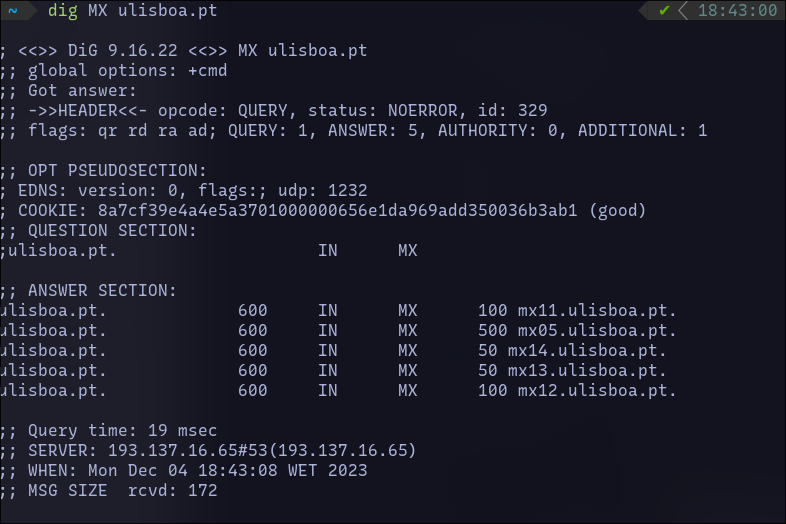
\includegraphics[width=5cm]{images/ulisboa.png} }}
    \qquad
    \subfloat[\centering UMinho]{{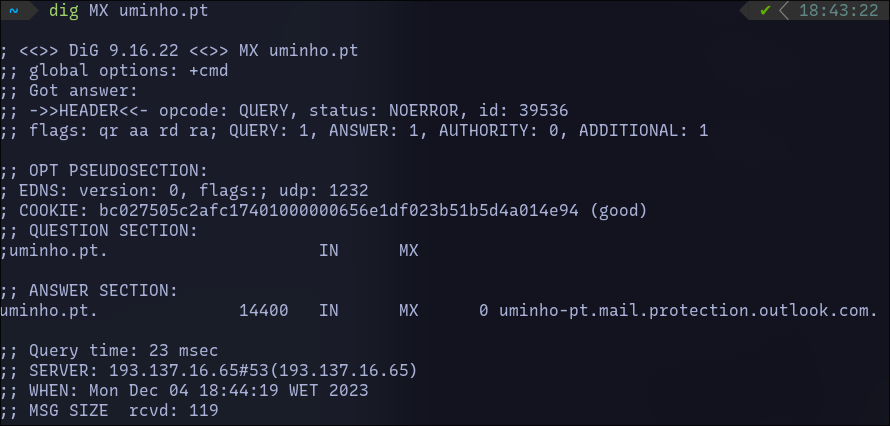
\includegraphics[width=5cm]{images/uminho.png} }}
\end{figure}

\end{document}
